% IEEE standard conference template; to be used with:
%   spconf.sty  - LaTeX style file, and
%   IEEEbib.bst - IEEE bibliography style file.
% --------------------------------------------------------------------------
\documentclass[twocolumn]{article} 
%\documentclass[letterpaper]{article} 
\usepackage{spconf,amsmath,amssymb,graphicx}
\usepackage[linesnumbered,ruled,vlined]{algorithm2e}
\usepackage{lmodern}
\usepackage{xcolor}
\usepackage{paralist}
\usepackage{caption}
%\usepackage{lipsum}

% Example definitions.
% --------------------
% nice symbols for real and complex numbers
\newcommand{\R}[0]{\mathbb{R}}
\newcommand{\C}[0]{\mathbb{C}}
\SetKwInput{KwInput}{Input}   

% bold paragraph titles
\newcommand{\mypar}[1]{{\bf #1.}}

% Title.
% ------
\title{Object Collision Detection via the GJK and BVH Algorithms}
%
% Single address.
% ---------------
\name{Mihai Zorca, Berke Egeli, Chris Müller, Liam van der Poel}
\address{Department of Computer Science\\ ETH Zurich, Switzerland}

\setlength{\textfloatsep}{5pt plus 4.0pt}

\setlength{\floatsep}{0pt plus 4.0pt}

%\captionsetup[figure]{font=footnotesize,labelfont=footnotesize}

\begin{document}

%\ninept
%
\maketitle
%

\begin{abstract} We present optimized implementations of two $3$D collision detection algorithms:  The Gilbert-Johnson-Keerthi Algorithm (GJK) and Bounding Volume Hierarchies (BVH). Previous papers consider only the speedup from simplifying GJK to perform intersection tests on convex shapes. Our contribution is to use SIMD vectorizations and other optimizations to achieve a speedup of $13.5\times$. BVH extends collision detection to general shapes. Our choice of k-DOP Bounding Volume (BV) quad trees allows efficient SIMD parallel intersection tests. Combined with half-precision floats we increased performance by up to $8.4\times$ compared to baseline.

%Describe in concise words what you do, why you do it (not necessarily
%in this order), and the main result. The abstract has to be
%self-contained and readable for a person in the general area. You
%should write the abstract last.
\end{abstract}

\section{Introduction}\label{sec:intro}

\mypar{Motivation} In computer graphics, video game design and related fields it is an important problem to quickly know if two objects intersect. For example, almost all video games require knowing when the player collides with an obstacle in their environment. This occurs very frequently and realistic interactions with obstacles are critical to immersive gameplay. 

\mypar{Contribution}
In this paper we present optimized implementations of two collision detection algorithms: Gilbert-Johnson-Keerthi (GJK) and Bounding volume hierarchy (BVH).

\mypar{Related work} 
The original GJK algorithm \cite{original_gjk} computes the minimum distance between two convex polytopes. A simplified version described by Muratori \cite{muratori} only tests if two objects intersect or not. This version is known as Boolean GJK. The major contribution is the \emph{DoSimplex} method which simplifies the algorithm given we do not need to explicitly compute the separation distance. Linahan \cite{gjk} provides an overview of the evolution of GJK, a geometric interpretation of the problem and proves that the optimizations proposed by Muratori are valid. However none of the previously mentioned papers consider the use of SIMD vectorisations and other optimizations to further increase performance.

Bounding Volume Hierarchies have been used in many fields of computer science to speed up collision detection \cite{simdop}.
Choosing a certain Bounding Volume means trading off tightness of fit and computation time for the intersection test.
Many different types of BVs have been tried: spheres \cite{hubbard}, AABBs \cite{aabbtree}, kDOPs \cite{kDOPtree}, OBBs \cite{obbtree} and even convex hull trees \cite{convexhulltree}.

The type of BV chosen for the tree and the number of children of each inner node also influence SIMD optimization potential.
In particular, the choice from \cite{simdop} of k-DOP BV quad trees allows efficient SIMD parallel intersection tests \cite{simdop}.

% Commented out as this isnt related work, this belongs in method section

%In this paper we also follow  this approach.
%Additionally, we also experiment with storing the kDOP BVs using only half-precision \texttt{F16C} floats.

%\begin{figure}\centering
%  \includegraphics[scale=0.33]{bvh-example.png}
%  \caption{Bounding Volume Hiecharchy with rectangle bounding %volumes}\label{bvh-example}
%\end{figure}

\section{Background Information}\label{sec:background}

This section presents the theoretical background on the two algorithms we implemented during this course: The Gilbert-Johnson-Keerthi Algorithm (GJK) and Bounding Volume Hierarchies (BVH).

\subsection{The Gilbert-Johnson-Keerthi (GJK) Algorithm}
GJK determines if two convex object $A, B$ intersect. 
First a few mathematical definitions are needed:
An Object is a non-empty set of points in 3d Euclidean space. 
The Minkowski difference $A - B$ of two objects is the object given by subtracting all points in $B$ from all points in $A$: $A - B := \{a - b : a \in A, b \in B\}$. 
An object $A$ is convex if and only if $(1 - \lambda)x + \lambda y \in A$ for all $x, y \in A$ and $\lambda \in [0, 1]$. 
A \textit{simplex} is generalization of the notion of a triangle to $n$ dimensions.

The algorithm uses the Theorem that $A, B$ intersect if and only if their Minkowski difference contains the origin \cite{bams/1183523140}. The pseudocode is given in Algorithm \ref{gjk}. 

This algorithm refers to the following functions: Support(A, D) which returns the furthest point on $A$ in direction $D$, and DoSimplex(S, D) which updates the simplex $S$, search direction $D$ and returns whether or not the updated simplex can contain the origin. The simplex $S$ is contained within our Minkowski sum $A - B$, so $S$ contains the origin only if $A-B$ does. 

\begin{algorithm}
\DontPrintSemicolon
 \KwInput{Object A, Object B, vector D}
 vector P = Support(A, D) - Support(B, -D) \\
 simplex s = {P} \\
 vector  D = -P \\
 \While{True} 
 {
 	vector P = Support(A, D) - Support(B, -D) \\
 	\If{dot(A, D) $< 0$:}
    {
       \Return False    \tcp*{No intersection}
    }
    s += {P} \\
    \If{DoSimplex(S, D):}
    {
       \Return True    \tcp*{Intersection}
    }
 }

\caption{GJK Pseudocode}
\label{gjk}
\end{algorithm}

\subsection{Bounding Volume Hierarchies (BVH)} 
\label{bvhbasics}

A limitation of GJK is that it can only be applied when both objects are convex. More general 3d objects are often represented by a mesh of geometric primitives, such as triangles, and are not necessarily convex. Bounding Volume Hierarchies (BVHs) are a data structure that allows efficient intersection tests in this more general case \cite{simdop}. Instead of doing intersection tests betwen all primitives of one object and all primitives of another, we recursively wrap the primitives with simple Bounding Volumes (BVs) such as rectangles, spheres or Discrete Oriented Polytopes (k-DOP). This results in a tree structure with bounding volumes as inner nodes, and the geometric primitives as the leaves. 

Our Bounding Volume is the k-DOP, and is defined using a fix set $\left\{d_1, \hdots, d_{k/2}\right\}$ of $k/2$ \textit{direction vectors} in $\mathbb{R}^3$. 
Any k-DOP is then represented using a vector $a \in \mathbb{R}^k$.
Concretely, it is the set $\left\{x \in \mathbb{R}^3 \ |\   \forall_{i \in \left[k/2\right]}: a_i \leq d_i^\top x \leq a_{2i} \right\}$.

Two k-DOPs (represented by the vectors $u,v \in \mathbb{R}^k$) \textbf{intersect }if and only if there does \textbf{not }exist an index $i$ such that $u_i < v_{2i}$ or $v_i < u_{2i}$.

To compute intersection of two BV trees, we traverse both trees and check if any volumes intersect. 
During traversal, if some parent volumes do not collide, their child volumes do not have to be tested. 
See Algorithm \ref{bvh} for the high-level traversal pseudocode \cite{simdop}.

\begin{algorithm}
\DontPrintSemicolon
 \If{$a$ and $b$ are both leaves}
 {
 	testTriangles($a$, $b$)
 }
 \ElseIf{$a$ is leaf}
 {
 	\For{each child $b_i$ of $b$}
 	{
 		\If{$a$ and $b_i$ intersect}
 		{
 			BVHintersect($a$, $b_i$)
 		}
 	}
 }
 \ElseIf{$b$ is leaf}
 {
 	\For{each child $a_i$ of $a$}
 	{
 		\If{$a_i$ and $b$ intersect}
 		{
 			BVHintersect($a_i$, $b$)
 		}
 	}
 }
 \Else
 {
 	\For{each child $a_i$ of $a$ and child $b_j$ of $b$}
 	{
 		\If{$a_i$ and $b_j$ intersect}
 		{
 			BVHintersect($a_i$, $b_j$)
 		}
 	}
 }
\caption{BVHintersect(BVHNode  a, BVHNode b)}
\label{bvh}
\end{algorithm}

\subsection{Cost Analysis}
Our cost measure is the number of additions, multiplications, and comparisons (and float conversions in the quantized BVH). 
We assume the compiler converts additions and multiplications into FMAs wherever it can. 
For both GJK and BVH the flop count is highly dependent on the topology of the two shapes we are comparing. 
We therefore have a flop counter that is dynamically incremented with the number of operations in each branch of the code. 
The cycle count is measured using the code from the assignments.

We defined the cost measure of GJK as the following:
\begin{equation*}
\resizebox{5.5cm}{!}{$
\begin{split}
C_{GJK}(n,m) & = (C_{mul}, C_{fma}, C_{cmp})(n,m) \\
& = n(m + 1)(C_{mul} + 2C_{fma} + C_{cmp})
\end{split}
$}
\end{equation*}
where $n$ is the total number of points of both of the input objects and  $m$ is the total number of iterations the GJK algorithm performs. 

%The number of iterations in the GJK algorithm depends on the shape of the objects and whether they intersect or not.
In order to ensure the convergence of the algorithm, we have limited the number of iterations to $100$ iterations. 
In each iteration of the algorithm, we traverse over the vertices of the input objects. 
Thus, GJK has the worst case complexity of $O(n)$.

We defined the cost measure of BVH as the following: 
\begin{equation*}
\resizebox{\linewidth}{!}{$
\begin{split}
& \ C_{BVH}\left(n_{ii}, n_{li}, t\right) \\
= & \ \left(C_{mul}, C_{fma}, C_{cmp}, C_{cvt}\right)\left(n_{ii}, n_{li}, t\right) \\
\leq & \  512 n_{ii}C_{cmp} + 128 n_{li} C_{cmp} + 50t \left(a C_{mul} + b C_{fma} + c C_{cmp}\right) + 16\left(n_{ii} + n_{li}\right) C_{cvt} %n(m + 1)(C_{mul} + 2C_{fma} + C_{cmp})
\end{split}
$}
\end{equation*}
where $n_{ii}$ is the no.~of inner-inner tests, $n_{li}$ is the no.~of leaf-inner tests, and $t$ is the no.~of triangle-triangle tests the BVH algorithm performs.
Finally, $a, b, c$ are constants s.t. $a + b + c = 1$ and $C_{cvt}=0$ for non-quantized code.
In practice, however, we measured the actual number of flops using counters in the code instead of relying on this model.

Asymptotically, the BVH trees are shallow, with a height expected in $O(\log n)$ (w.r.t. $n$, the number of triangles in the original mesh).
However, in the worst possible case, no triangles intersect but all BVs overlap, so all nodes of the tree must be tested. 
As each tree has less than $2n$ nodes and each node is tested against at most $4$ other nodes, the worst case traversal complexity is in $O(n)$.

%Give a short, self-contained summary of necessary
%background information on the algorithm or application that you then later optimize including a cost analysis.
%
%For example, assume you present an
%implementation of FFT algorithms. You could organize into DFT
%definition, FFTs considered, and cost analysis. The goal of the
%background section is to make the paper self-contained for an audience
%as large as possible. As in every section
%you start with a very brief overview of the section. Here it could be as follows: In this section
%we formally define the discrete Fourier transform, introduce the algorithms we use
%and perform a cost analysis.
%
%\mypar{Discrete Fourier Transform}
%Precisely define the transform so I understand it even if I have never
%seen it before.
%
%\mypar{Fast Fourier Transforms}
%Explain the algorithm you use.
%
%\mypar{Cost Analysis}
%First define you cost measure (what you count) and then compute or determine on other ways the
%cost as explained in class. In the end you will likely consolidate it into one number (e.g., adds/mults/comparisons) but be aware of major imbalances as they affect the peak performance..
%
%Also state what is known about the complexity (asymptotic usually)
%about your problem (including citations).


\section{GJK \& BVH Implementation}\label{sec:yourmethod}
This section explains the baseline implementation and optimization details for our two algorithms. 
\subsection{GJK Baseline Implementation}
\label{subsec:gjkbase}
Baseline GJK algorithm takes two 3D objects as inputs. An object is represented by a struct that stores an $N \times 3$ matrix (where $N$ is the number of vertices of the object). We refer to this as the Array of Structures (AoS) format. This is the most intuitive and common way that shapes represent their data.

The baseline implementation of GJK mainly consists of multiple Support functions and the DoSimplex function.

%The Support function returns a set of point on an object based on a search direction.
%The vertices of the simplex are calculated by applying Minkowski difference to these points.
%Initially, the search direction is initialized arbitrarily, but later it is updated by the DoSimplex method.
%DoSimplex function applies plane tests to the simplex and tries to determine the new search direction towards the origin.
%We iteratively update the simplex and the search direction until either the simplex encloses the origin or we conclude that it can never enclose the origin.

\mypar{Support Function}
A Support function takes an object and a search direction as input. It returns the vertex on the object that lies farthest away in the search direction. To do this, we iterate over every vertex of the object and calculate the dot product between each vertex and the search direction. We then take the argmax of these values.

\mypar{DoSimplex Function}
The DoSimplex function takes a simplex and a search direction as input. Based on the number of points in the simplex we apply the corresponding plane tests for a line, triangle or tetrahedron. These tests update the search direction and the simplex. We detect a collision when we have a tetrahedron simplex and it contains the origin. Otherwise we either continue the search, or return that we will never contain the origin.

\mypar{Profiling}
We used DTrace tool to profile the baseline implementation. Profiling showed that GJK spends between 65\% and 98\% of the total execution inside Support functions. Execution time of the Support functions scales with input size, for the DoSimplex function it remains constant. 

\mypar{Locality}
The GJK algorithm benefits from spatial locality. GJK algorithm also exhibits temporal locality because we access the same set of points in each iteration. However, depending on the size of the input objects, the algorithm can not properly exploit this locality. If the objects do not fit in the cache, they start evicting each other. Thus, they need to be brought back from main memory to caches. Unfortunately, due to the iterative nature of the algorithm, it is not possible to reorder or parallelize the support calls in a way that avoids capacity misses. 

\mypar{Bandwidth/Data Transfer Analysis}
The bandwidth/data trasfer analysis showed that baseline GJK is compute bound for all of the input sizes used in the experiments. 

The analysis showed us that the main bottleneck of GJK are the Support functions, so this was where we focused the optimization effort. Cache optimizations are not feasible due to iterative nature of the algorithm. Finally, GJK can benefit greatly from SIMD intrinsics because it is compute bound and the Support functions have a greatly parallelizable nature.

\subsection{GJK Standard C Optimizations}
\mypar{Block Optimizations}
Inside the support function, the computations in the main loop are independent from previous iterations. This allows basic block optimizations. We applied scalar replacement, loop unrolling and accumulators to exploit instruction level parallelism (ILP) in the loop. We tested the algorithm with two different loop unrolls, 2 and 8.

\mypar{Method Inlining and Joint Loop Optimization}
Inside the main loop of the GJK algorithm, we sequentially call a support function on each input object. Let the inputs have $N$ and $M$ vertices respectively. This gives $N + M$ iterations in the support functions. We can reduce the total number of iterations by manually inlining the support calls inside GJK and joining the two loops from the support functions. This trick splits the loops into three parts. First we iterate over both objects for $min\{N, M\}$ iterations. Second we complete the iterations for the first object. Third we complete the iterations for the second object. The first loop fully iterates over the smaller object, so we only enter the second or the third loop. This inlining reduces the total number of iterations to $max\{N, M\}$.

\subsection{GJK SIMD Optimizations}
\mypar{Vectorization with AVX2 Intrinsics}
Vectorization allows us to do the dot product and argmax operations in the support functions in parallel. First load the object vertices into 
128-bit vectors. Then append two 128-bit vectors into a 256-bit vector. Calculate two dot products in parallel using the $\_mm256\_dp\_ps$ intrinsic. Store the results of 8 dot products in a single 256-bit vector. Finally, apply one argmax operation to get the maximum dot product. The $i$'th slot of the result vector contains the maximum dot product of all dot products in the $i$'th slot of the input vector. Likewise we vectorize the branching in the argmin operation. Finally, outside of the loop we apply an argmax over the maximum dot product vector.

AoS format and 3D points limit our ability to vectorize. We did not use AVX/AVX512 intrinsics for the main computations as while they would let us vectorize the multiplication in the dot product, we would still have to extract the values inside the vector to do the scalar addition of three floats. This overhead negated any speedup from the vectorization. Due to AoS format, we also had to load each vertex to 128-bit vectors because we could only separately calculate the dot product of 4 consecutive floating point numbers in the 256-bit vectors. 

\mypar{Conversion to Structure of Arrays (SoA) Format and Vectorization with AVX512 Intrinsics}
Vectorization with AoS format did not provide significant speedup because of the limitations outlined in the previous section. So we changed the representation of our vertices to SoA format which is more suitable for vectorization. We could now directly use AVX512 intrinsics without having to shuffle or combine data. In SoA format, each coordinate of a vertex is stored in three different arrays. We load each coordinate into three 512-bit vectors separately. We calculate the dot product as shown in Algorithm ~\ref{dot product}. Then we calculate the argmax as in the AVX2 version. This implementation provides us significant speedup because we are able to calculate 16 dot products in parallel without shuffling the data.

\mypar{Strength Reduction in Index Calculation}
We achieved substantial speedup by applying strength reduction to the index calculation. In our initial AVX512 implementation, we were using \_mm512\_set\_epi32 to calculate the indices for argmax operation. Taking this operation outside of the main loop and replacing it with \_mm512\_add\_epi32 inside the loop allowed us to achieve our maximum speedup.

\begin{algorithm}
\DontPrintSemicolon
 \KwInput{vector X, vector Y, vector Z, vector D[0], vector D[1], vector D[2]} 
 tmp\_0 = \_mm512\_mul\_ps(X, D[0]) \\
 tmp\_1 = \_mm512\_fmadd\_ps(D[1], Y, tmp\_0) \\
 dp = \_mm512\_fmadd\_ps(D[2], Z, tmp\_1) \\
\caption{AVX512 dot product}
\label{dot product}
\end{algorithm}

\subsection{BVH Baseline Implementation}
Baseline BVH algorithm takes two $3$D objects as input.
These objects are represented as an AoS triangle mesh: a struct that stores an array of triangles.
Triangles in turn are just arrays of $3$D points.
AoS format is chosen for the same reasons as mentioned in \ref{subsec:gjkbase}.

For both input objects, first the BVH tree has to be constructed.
For this tree construction we follow the SIMDop paper \cite{simdop} and use the \textit{Batch Neural Gas} algorithm described in \cite{neural}.
Tree construction can be regarded as a "pre-processing" step, as it only has to be performed once, independent of the number of scene objects / performed collision tests.
For this reason, we focus our optimization efforts not on this tree construction, but rather on the subsequent tree traversal.

Following Algorithm \ref{bvh}, our intersection test is a recursive procedure that takes two BVH tree nodes as input. 
Each BVH node is either an inner node, in which case it stores the k-DOP bounding volumes of its 4 children. 
Or it is a leaf, in which case it is simply a tagged pointer to a triangle array (of at least 1 and at most 4 triangles).

Its three main components are \textit{triangle-triangle} tests, \textit{leaf node  - inner node} tests and \textit{inner node - inner node} tests.

\mypar{Inner-Inner Tests} This is the core case, when an inner node $n_a$ from tree $a$ overlaps with an inner node $n_b$ from tree $b$.
In this case, we have to test for each child of $n_a$, if its k-DOP bounding volume overlaps with any k-DOP bounding a child of $n_b$.
As each inner node has 4 children, this results in 16 k-DOP overlap tests.
Recalling section \ref{bvhbasics}, testing k-DOP overlap is a series of at most $k$ floating point compares.
However, if we find an index $i$ then we can stop early and conclude disjointness. 
This becomes important later, as vectorized implementations lack this "early-stopping" ability and always perform all $k$ comparisons.

\mypar{Leaf-Inner Tests}
This happens when we reach a leaf in one tree, but still consider inner nodes in the other tree. 
The only difference to the \textit{inner-inner} case is that we test one k-DOP (bounding the leaf) vs. 4 k-DOPs of the children of the inner node.

\mypar{Leaf-Leaf Tests}
Here, we have reached leaves in both trees, so we can directly test the triangles both leaves point to using the standard Möller triangle-triangle test \cite{moeller}.
As leaves point to between 1 and 4 triangles, up to 16 such tests have to be performed.

\textbf{Note: } Our attempt to vectorize the Triangle-Triangle case was not successful.
Möller's algorithm is very unsuitable to vectorization, as it is mostly comprised of case distinctions.
This, together with the profiling results, made us focus our optimization efforts on traversal and the Leaf-Inner and Inner-Inner Tests.

\mypar{Profiling}
We implemented various counters in the BVH code, which allowed us to profile the implementation.
Profiling showed that BVH spends between $70\%$ and $95\%$ on tree traversal. 
The remaining time is spent in the leaf triangle-triangle tests.

\mypar{Locality} 
As can be expected for a tree traversal algorithm (read: chasing pointers), locality is poor. 
After a node has been fetched and one of the three test cases is applied, this node will never be tested again. 
Therefore, almost no temporal locality is available.
The only exception to this is the leaf-inner case: the leaf node of one tree can be tested against multiple nodes of the other tree.
Still, at most $O(1)$ memory - that of that one leaf-parent node - will have temporal locality, independent of input sizes.
A node stores the kDOPs of all 4 children in contiguous memory and leaves point to a contiguous triangle-array, therefore some spacial locality exists. 
However, the location of different nodes is arbitrary and they have to be fetched via pointer access.
So again, at most $O(1)$ memory (of $2$ nodes) has spacial locality at any given time. 

\mypar{Bandwidth/Data Transfer Analysis}
Like all aspects of this algorithm, operational intensity depends on the underlying scene geometry. 
Specifically, the ratio of triangle-triangle tests to inner-node tree traversal tests is relevant here. 
Over all, the baseline operational intensity is between $\approx 0.15$ and $\approx 0.45$.
Further, while operational intensity depends on the scene geometry, it does \textbf{not} depend on input size: almost all cache misses we incur are compulsory misses.

\subsection{BVH SIMD Optimizations}
We vectorize both inner-inner and leaf-inner tests.
The main idea for vectorizing comes from \cite{simdop}. 

\mypar{Inner-Inner Tests} Here we aim to perform all 16 possible tests at once.
The $4$ kDOP vectors in an inner node are stored contiguously in a $k \times 4$ float $2D$-array.
This means, a single \texttt{\_mm\_512\_load\_ps()} can load the kDOP values for $4$ DOP directions for all four children into one vector $v$.
After this, for each of the $k/2$ DOP directions, we extract a suitable permutation for comparing the intervals using a \texttt{\_mm512\_permutexvar\_ps()}  instruction.
Table \ref{fig:dopperm} shows the permutations 
inside the registers. 
The two registers can then be compared via \texttt{\_mm512\_cmp\_ps\_mask()} and each of the resulting $16$ bits indicates (non-)overlap along the current direction of one of the $16$ pairs of children.

\begin{table}
\begin{center}
\resizebox{8.5cm}{!}{
\begin{tabular}{ | c | c | c | c | c | c | c | c | c | c | c | c | c | c | c | c | }
\hline
$a_1$ & $a_2$ & $a_3$ & $a_4$ & $a_1$ & $a_2$ & $a_3$ & $a_4$ & $a_1$ & $a_2$ & $a_3$ & $a_4$ & $a_1$ & $a_2$ & $a_3$ & $a_4$ \\
\hline  
\multicolumn{1}{c}{}\\
\multicolumn{1}{c}{}\\
\hline
$b_1$ & $b_1$ & $b_1$ & $b_1$ & $b_2$ & $b_2$ & $b_2$ & $b_2$ & $b_3$ & $b_3$ & $b_3$ & $b_3$ & $b_4$ & $b_4$ & $b_4$ & $b_4$ \\
 \hline
\end{tabular}
}
\end{center}
\caption{Permutation of the values for the four DOPs $a_1,...,a_4$ of a node $A$ and the four DOPs $b_1,...,b_4$ of a node $B$ to produce a single $512$ Bit AVX register for comparing all $4\times 4$ possible combinations \cite{simdop}.}
\label{fig:dopperm}
\end{table}

\mypar{Leaf-Inner Tests} The approach is similar to the Inner-Inner vectorization, except that now we test one kDOP against $4$ kDOPs. 
To fully exploit the AVX-$512$ registers, we now test all four kDOP pairs \textbf{along four DOP directions} at the same time.
An non-obvious consequence is that during loading, the new permutations no longer cross AVX lanes. 
Thus, the faster \texttt{\_mm512\_permute\_ps()} instruction can be used.

\subsection{BVH Quantization via Half-Precision Floats}
The \texttt{x86} extension set called \texttt{F16C} provides hardware support for converting to and from $16$ bit half-precision floats. 
As our tree traversal is memory-bound, we aim to reduce the memory bandwidth by storing the DOP values using $16$ bit half floats. 
Each register now fits $32$ such half floats.
However, no half-precision arithmetic operations are supported, so the values have to be converted back to $32$ bit floats.
The conversion happens via two steps: 
\begin{compactitem}
\item An \texttt{\_mm512\_extracti64x4\_epi64()} instruction and the \texttt{\_mm512\_cvtph\_ps()} conversion for the high $16$ half floats and
\item A no-op cast \texttt{\_mm512\_castsi512\_si256()} followed by \texttt{\_mm512\_cvtph\_ps()} for the low $16$ half floats 
\end{compactitem}
Aside from this additional conversion overhead, all other vectorization ideas translate very well.
As each load takes $32$ half floats, we also unroll the loop once, even though registers and ports are already filled in a single iteration.

Due to less precise BV fit, there is a slight increase in false positives for triangle-triangle tests (non-overlapping triangles tested due to overlapping BVs).
However, the faster traversal most often makes up for this and we still see a speedup when using the quantized implementation.

\subsection{BVH Specialized Recursion}
Observe that as we traverse the trees, once we reach a leaf in either tree we will not visit an inner node in that tree again until we back-track from our current recursion level.
We exploit this and build two recursive functions: the general case seen in Algorithm \ref{bvh} and the specialized case, where the inner-inner case is not present.
The specialized function has fewer parameters (only $2$ pointers and one int vs. $4$ pointers and $2$ ints in the general case).
Further, we don't have to run an always negative test for the inner-inner case.
We apply this to both the vectorized and quantized versions.

% Now comes the ``beef'' of the paper, where you explain what you
% did. Again, organize it in paragraphs with titles. As in every section
% you start with a very brief overview of the section.

% For this course, explain all the optimizations you performed. This mean, you first very briefly
% explain the baseline implementation, then go through locality and other optimizations, and finally SSE (every project will be slightly different of course). Show or mention relevant analysis or assumptions. A few examples: 1) Profiling may lead you to optimize one part first; 2) bandwidth plus data transfer analysis may show that it is memory bound; 3) it may be too hard to implement the algorithm in full generality: make assumptions and state them (e.g., we assume $n$ is divisible by 4; or, we consider only one type of input image); 4) explain how certain data accesses have poor locality. Generally, any type of analysis adds value to your work.

% As important as the final results is to show that you took a structured, organized approach to the optimization and that you explain why you did what you did.

% Mention and cite any external resources including library or other code.

% Good visuals or even brief code snippets to illustrate what you did are good. Pasting large amounts of code to fill the space is not good.

%\begin{figure}[htp]
%   \centering
%   \subfigure{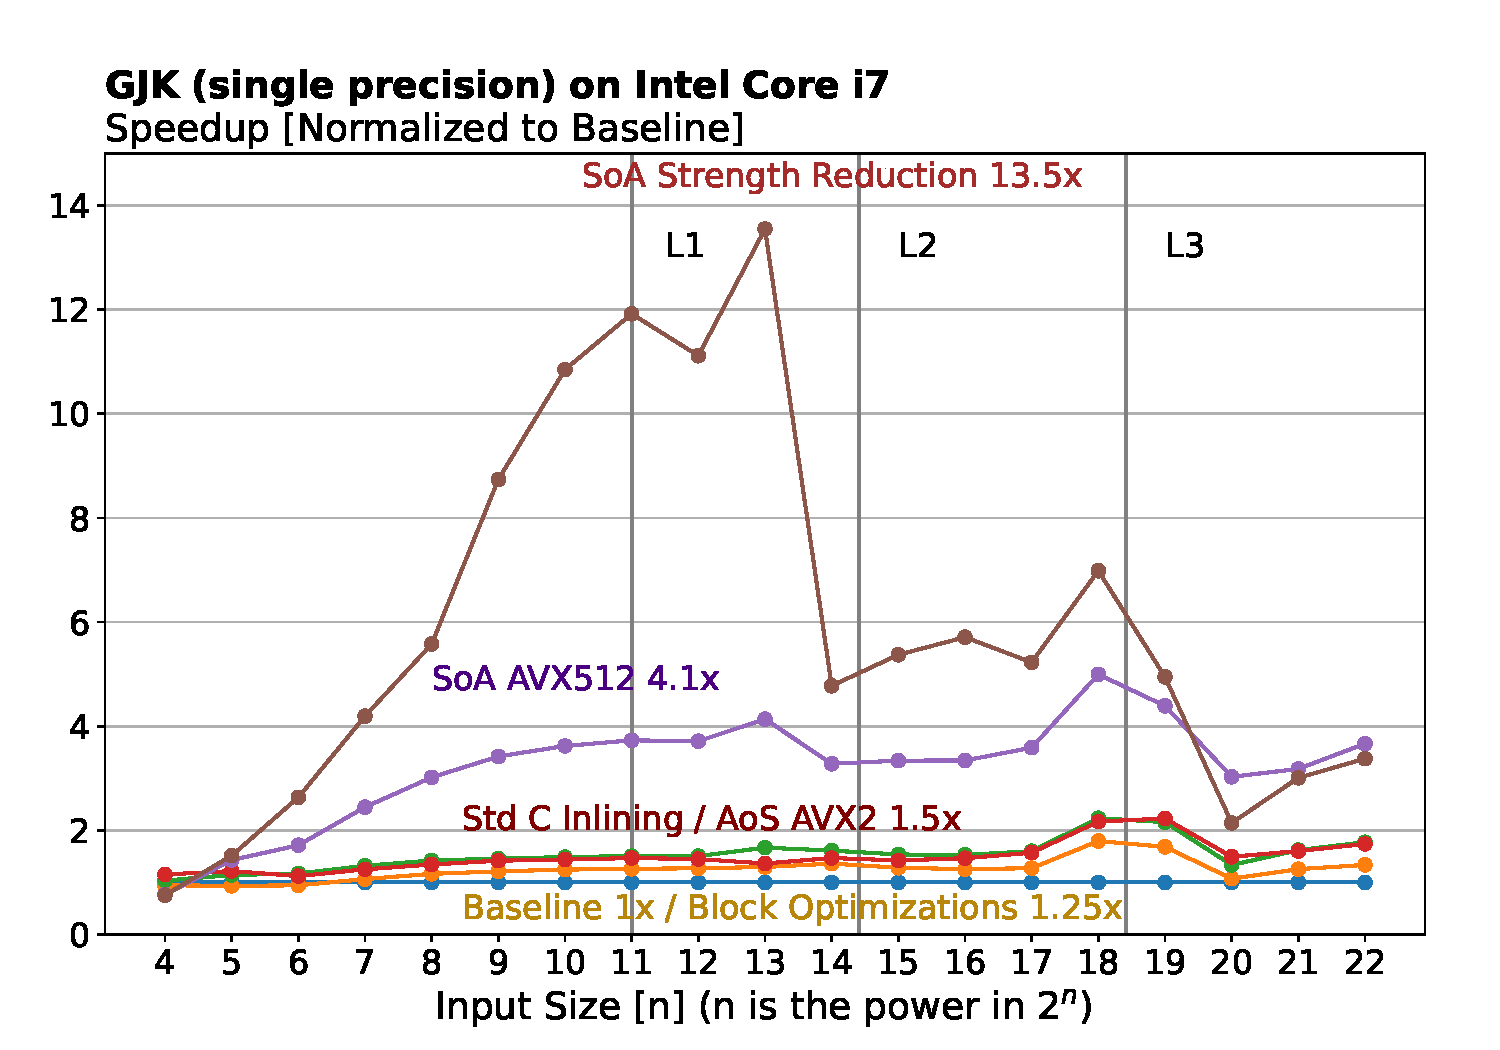
\includegraphics[scale=0.33pt]{gjk_speedup.pdf}}\quad
%   \subfigure{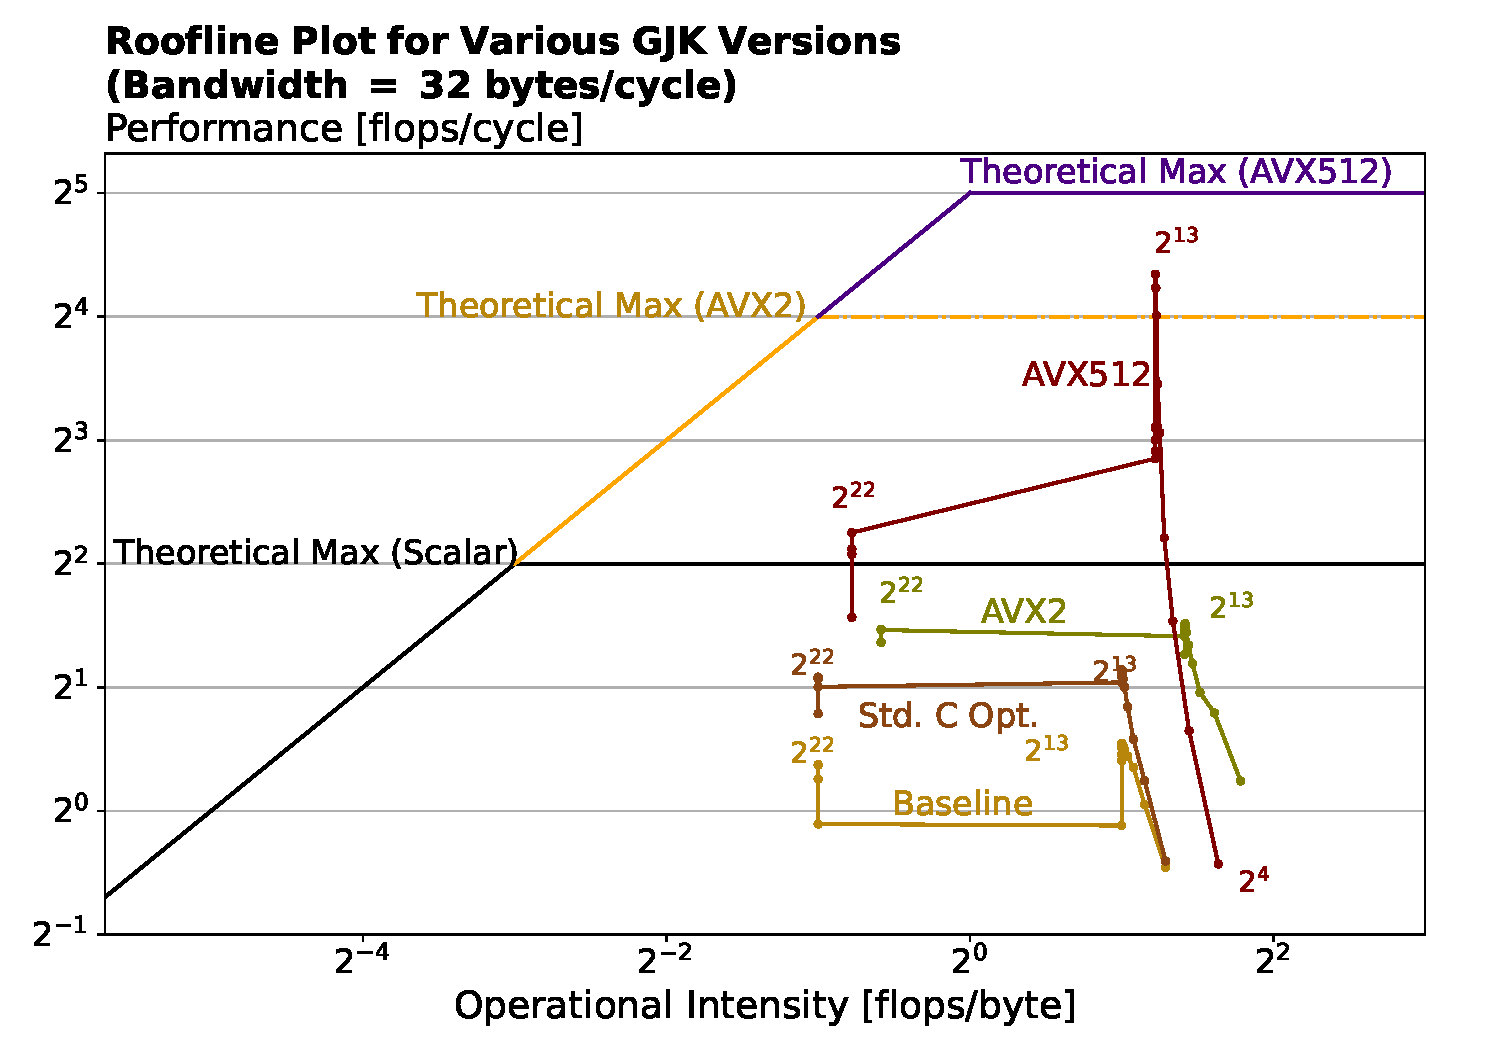
\includegraphics[scale=0.33pt]{gjk_roofline.pdf}}
%   \caption{ Speedup and Roofline plots for GJK. AVX2 implementation has around 15\% and AVX512 has around 30\% more flops. 
%   \label{gjkspeedup_roofline}}
%\end{figure}

\section{Experimental Results}\label{sec:exp}

This section gives the hardware and software specifications for the machines used to run GJK and BVH respectively, as well as the experimental results of the optimizations described in the Method section. 

\mypar{Experimental setup for GJK}

We conducted our experiments for GJK using an Intel® Core™ i7-1068NG7 processor which uses the Icelake architecture. It has a base frequency of 2.3 GHz. The cache sizes for L1, L2 and L3 caches are 80KiB (32 KiB \textbf{I} + 48 KiB \textbf{D}), 512KiB and 8MiB (shared) respectively. L1 and L2 caches are 8 way associative, and L3 cache is 16 way associative. To compile our code, we used GCC version 10.2.0. The optimization flags we used are: \texttt{-std=c11 -O3 -march=icelake-client -ffast-math}. The experiments were conducted using \textbf{cold} caches.

As inputs we generated two spheres of equal sizes. The sizes of the each sphere ranged from 16 vertices to 2\textsuperscript{22}. GJK algorithm only needs the convex hull of input objects to operate. Therefore, all of the points of the spheres were on the surface.


\mypar{Results (GJK)}
Fig.~\ref{gjkspeedup} shows the speedup each optimization achieved compared to the baseline GJK implementation. 
It appears that standard C optimizations failed to improve GJK algorithm significantly. 
The block optimizations provide 25\% speedup and combining block optimizations with the method inlining/joint loop trick brings us up to ~45-50\% total speedup. 
The mediocre speedup is caused by the dependencies in our bottleneck. 
When we check Fig.~\ref{gjkperformancestdc} we can see that our potential peak performance is actually not that high. 
In the optimized versions, inside support function loop, we do 1 multiplication, 2 FMAs and 1 comparison operation. 
All of these instructions create a Read After Write (RAW) dependency. Just by considering instruction mix, the peak performance drops from 4 flops/cycle to 3 flops/cycle. 
When we further consider the instruction dependencies, we observed that we issue 48 flops in 19 cycles per iteration of the loop. This further brings our potential peak performance to 2.52 flops/cycle. 
Unfortunately, our standard C optimized versions failed to reach this peak. 
This suggests that there are still possible avenues of optimization in these versions.

\begin{figure}[!ht]
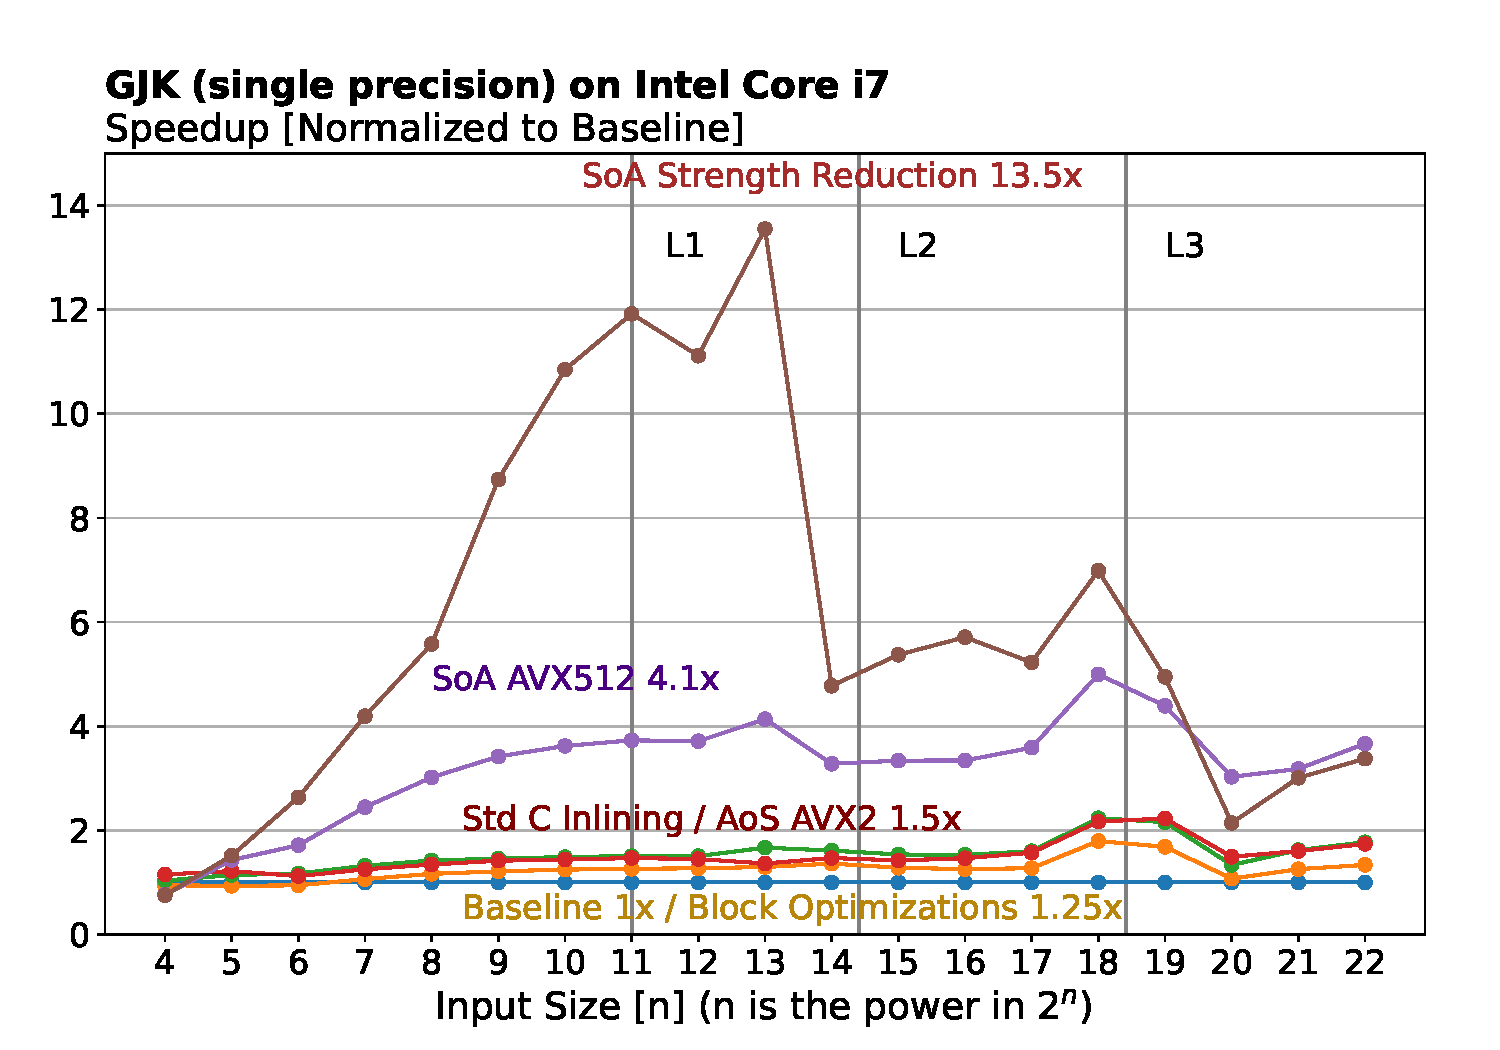
\includegraphics[width=\linewidth]{gjk_speedup.pdf}
\caption{Speedup plot of all versions of GJK algorithm. Execution time is measured in cycles. The execution times are normalized to the baseline runtime.}
\label{gjkspeedup}
\end{figure}

Vectorization with AVX2 intrinsics failed to achieve any meaningful speedup.
The vectorization limitations from AoS format and the subsequent shuffling/combining of smaller vectors hurt the speed of the algorithm. 
When we look at Fig.~\ref{gjkperformanceavx}, AVX2 implementation seems to have a slightly better performance compared to standard C versions, however this is misleading since we simply do 15\% more computations in AVX2 version to do the same work as in standard C versions.

\begin{figure}[!ht]
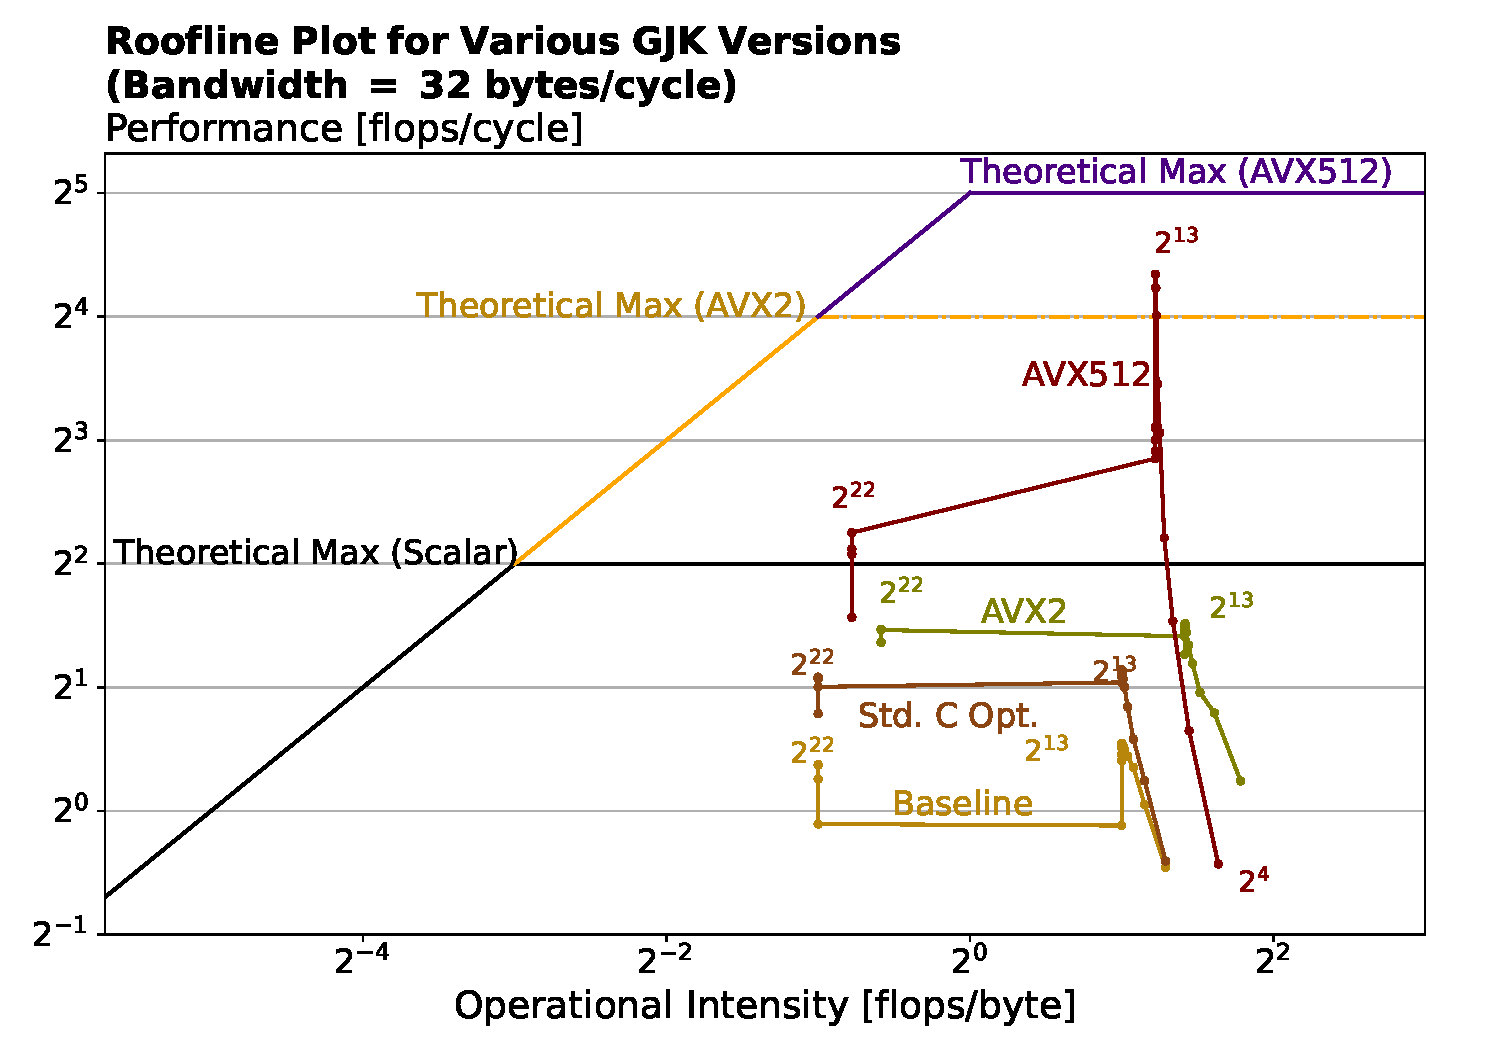
\includegraphics[width=\linewidth]{gjk_roofline.pdf}
\caption{ Roofline plots for GJK. AVX2 version has around 15\% and AVX512 has around 30\% more flops.}
\label{gjkroofline}
\end{figure}

Our initial AVX512 implementation without strength reduction achieved more than 2x speedup compared to AVX2 implementation with strength reduction.
Conversion to SoA format greatly benefited the vectorized implementations because it enabled us to use larger vectors. We further gained ~3x speedup when we applied strength reduction to the index calculations in the AVX512 implementations. 
This brought us to our peak performance of 13.5x speedup compared to the baseline implementation. 
As can be seen from Fig.~\ref{gjkperformanceavx}, our maximum performance is close to the peak performance of 22.4 flops/cycle we get when we consider the instruction mix. 
We again use 1 multiplication, 2 FMAs and 1 comparison operation in our bottleneck loop. 
However, in the vectorized implementations we also use an additional maximum operation. 
This means that when we consider only the instruction mix, we issue 112 flops in 5 cycles. 
We are likely to be even closer to real peak performance when we consider the instruction dependencies as well.

\begin{figure}[!ht]
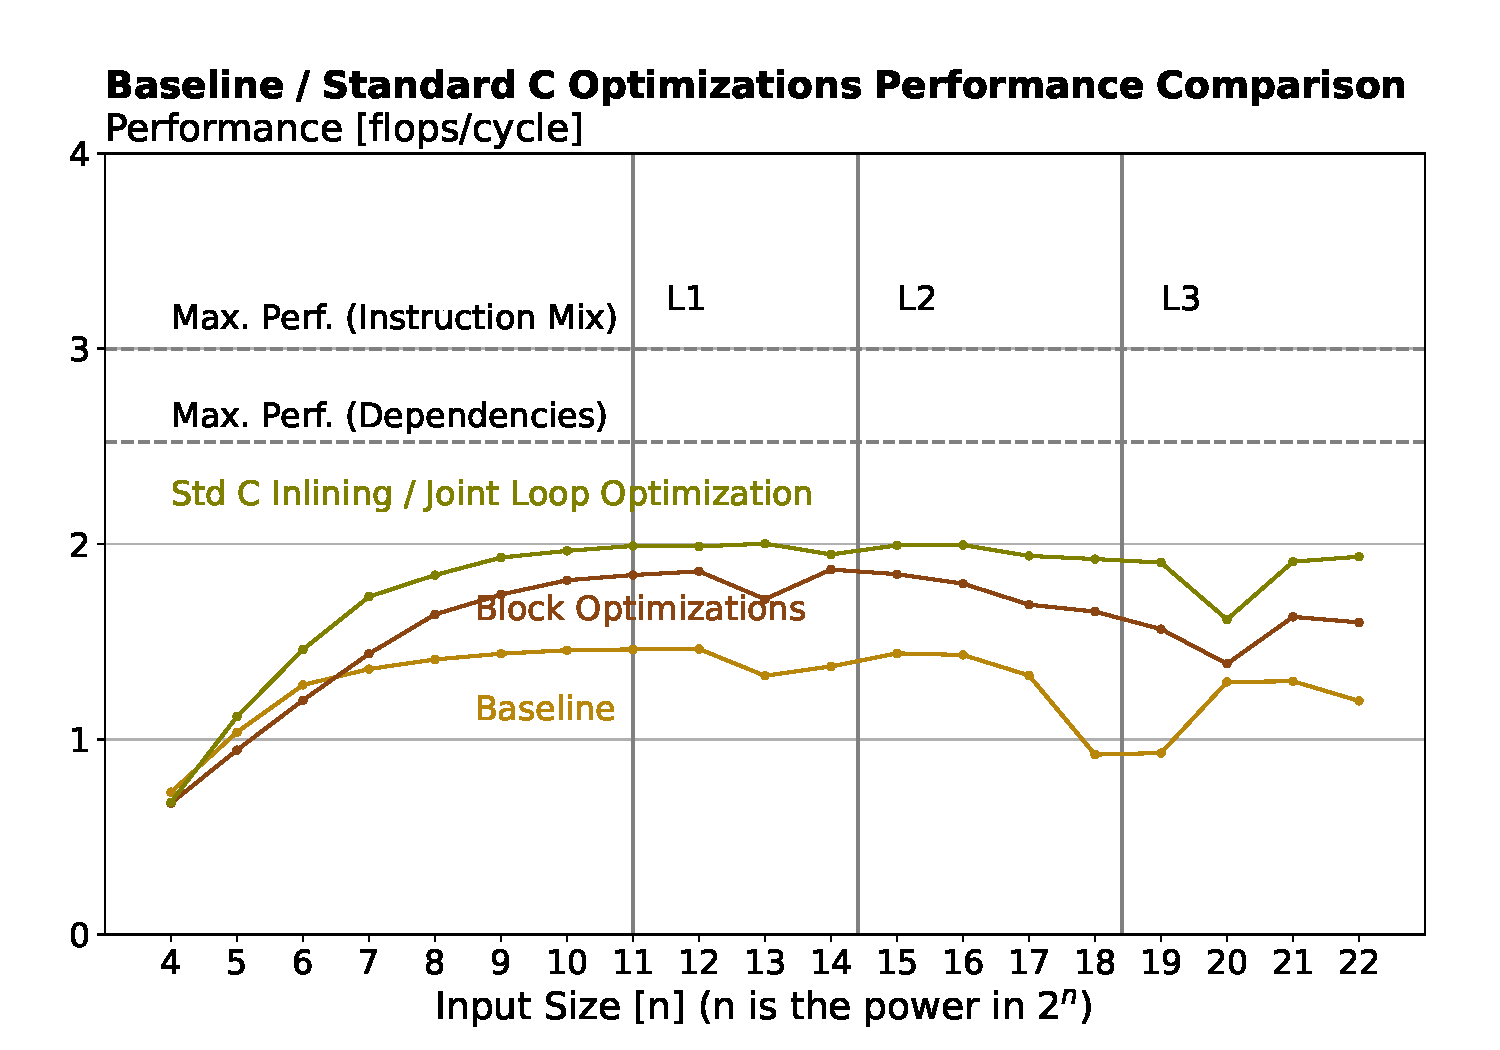
\includegraphics[width=\linewidth]{gjk_performance_stdc.pdf}
\caption{Performance plots for scalar implementations of GJK.  The operation counts are roughly the same. }
\label{gjkperformancestdc}
\end{figure}

In our bandwidth/data transfer analysis, we mentioned that the baseline GJK implementation was compute bound. From Fig.~\ref{gjkroofline} it can be seen that, this turned out to be true for almost all of our implementations.
Only when the data does not fit in cache the AVX512 implementations become memory bound. 
This is caused by the shift in operational intensity when the data does not fit in cache. 
Our operational intensity decreases because we iterate over the same two objects over and over again. 
When the objects do not fit in cache we have to repeatedly bring them into caches, hence, more data transfers between L3 cache and main memory.

\begin{figure}[!ht]
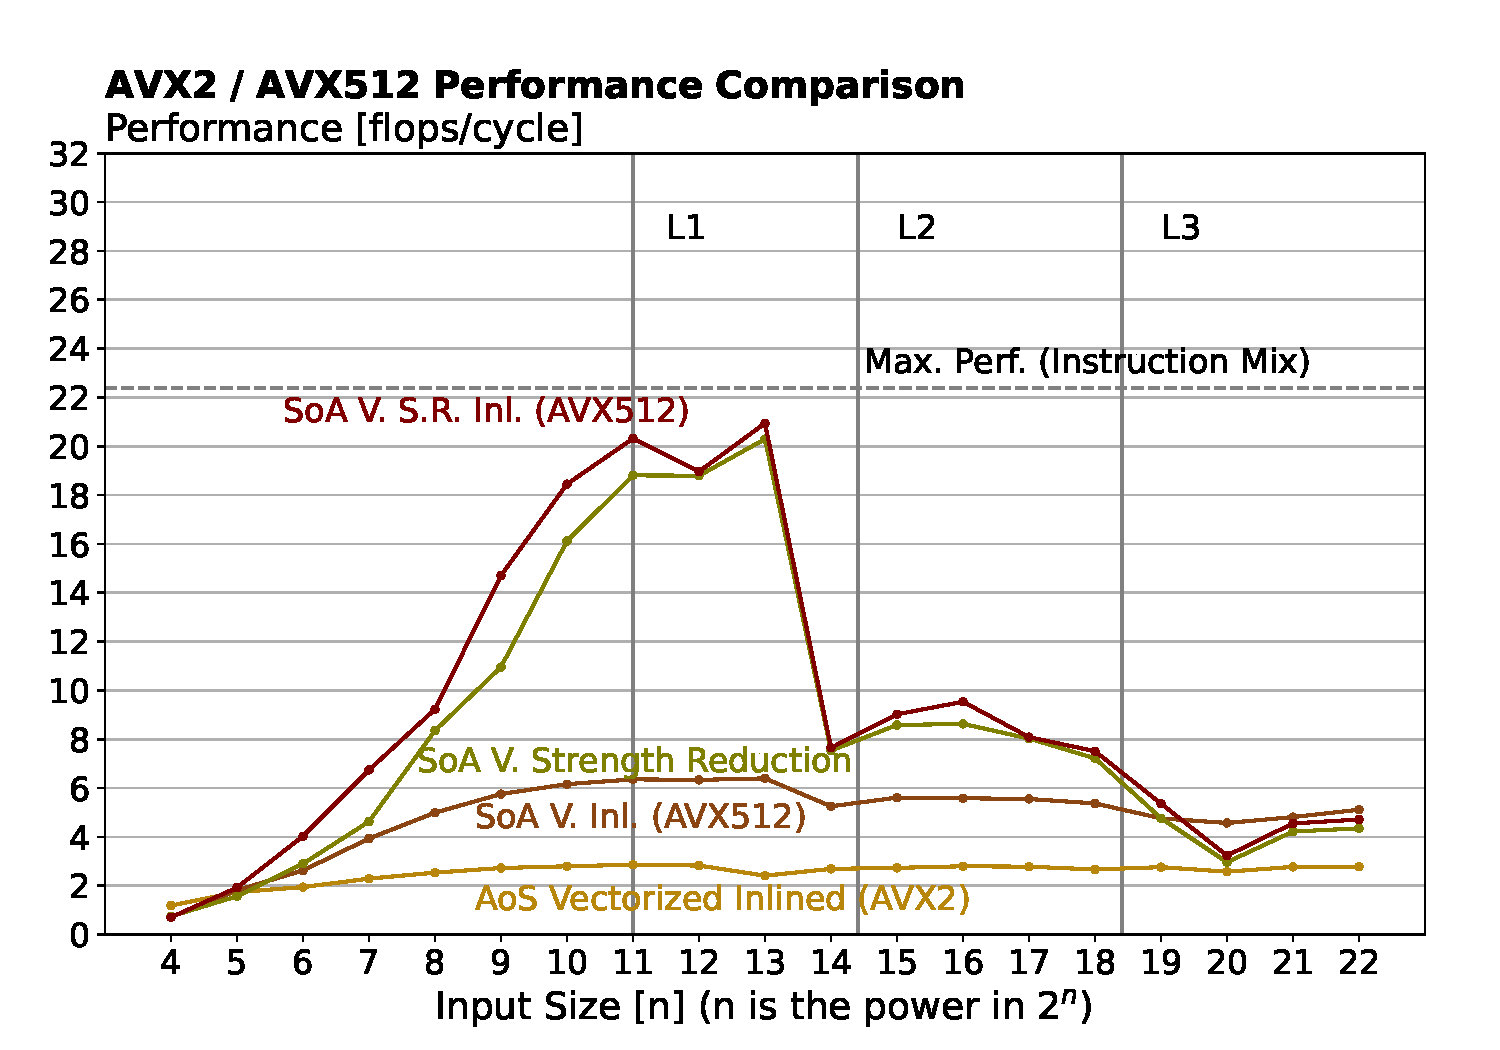
\includegraphics[width=\linewidth]{gjk_performance_avx.pdf}
\caption{Performance plots for vectorized implementations of GJK.  The operation count of AVX512 versions is roughly 10\% more than operation of AVX2 version. }
\label{gjkperformanceavx}
\end{figure}

%\begin{figure*}
%  \subfigure{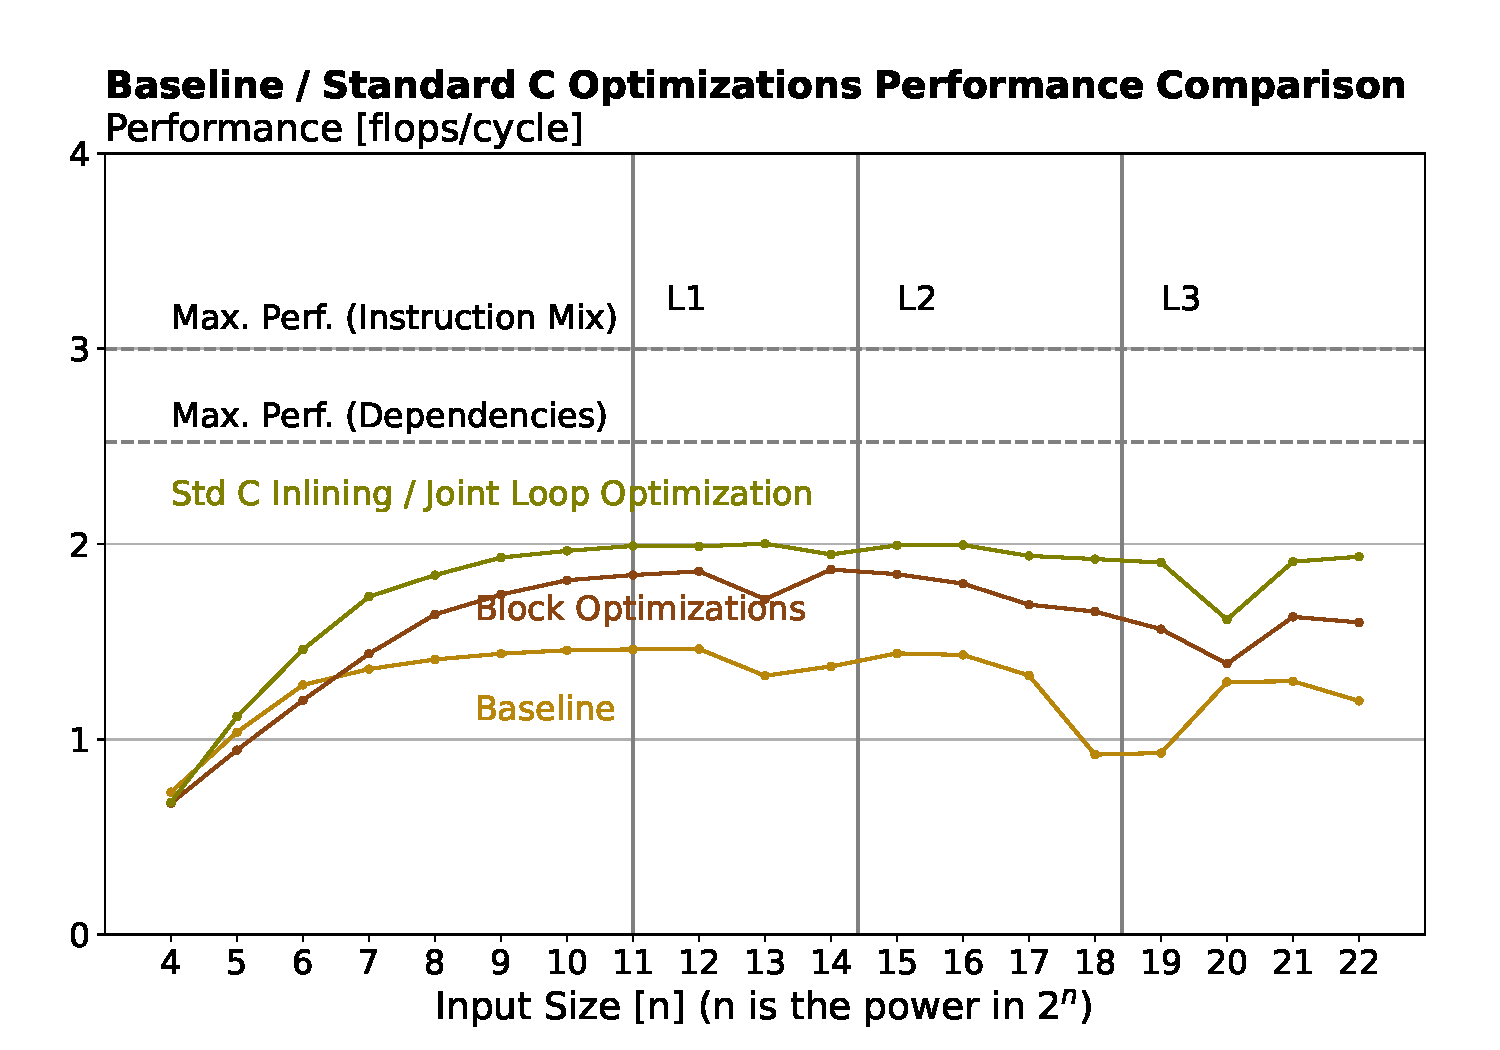
\includegraphics[scale=0.33]{gjk_performance_stdc.pdf}}
%    \quad
%  \subfigure{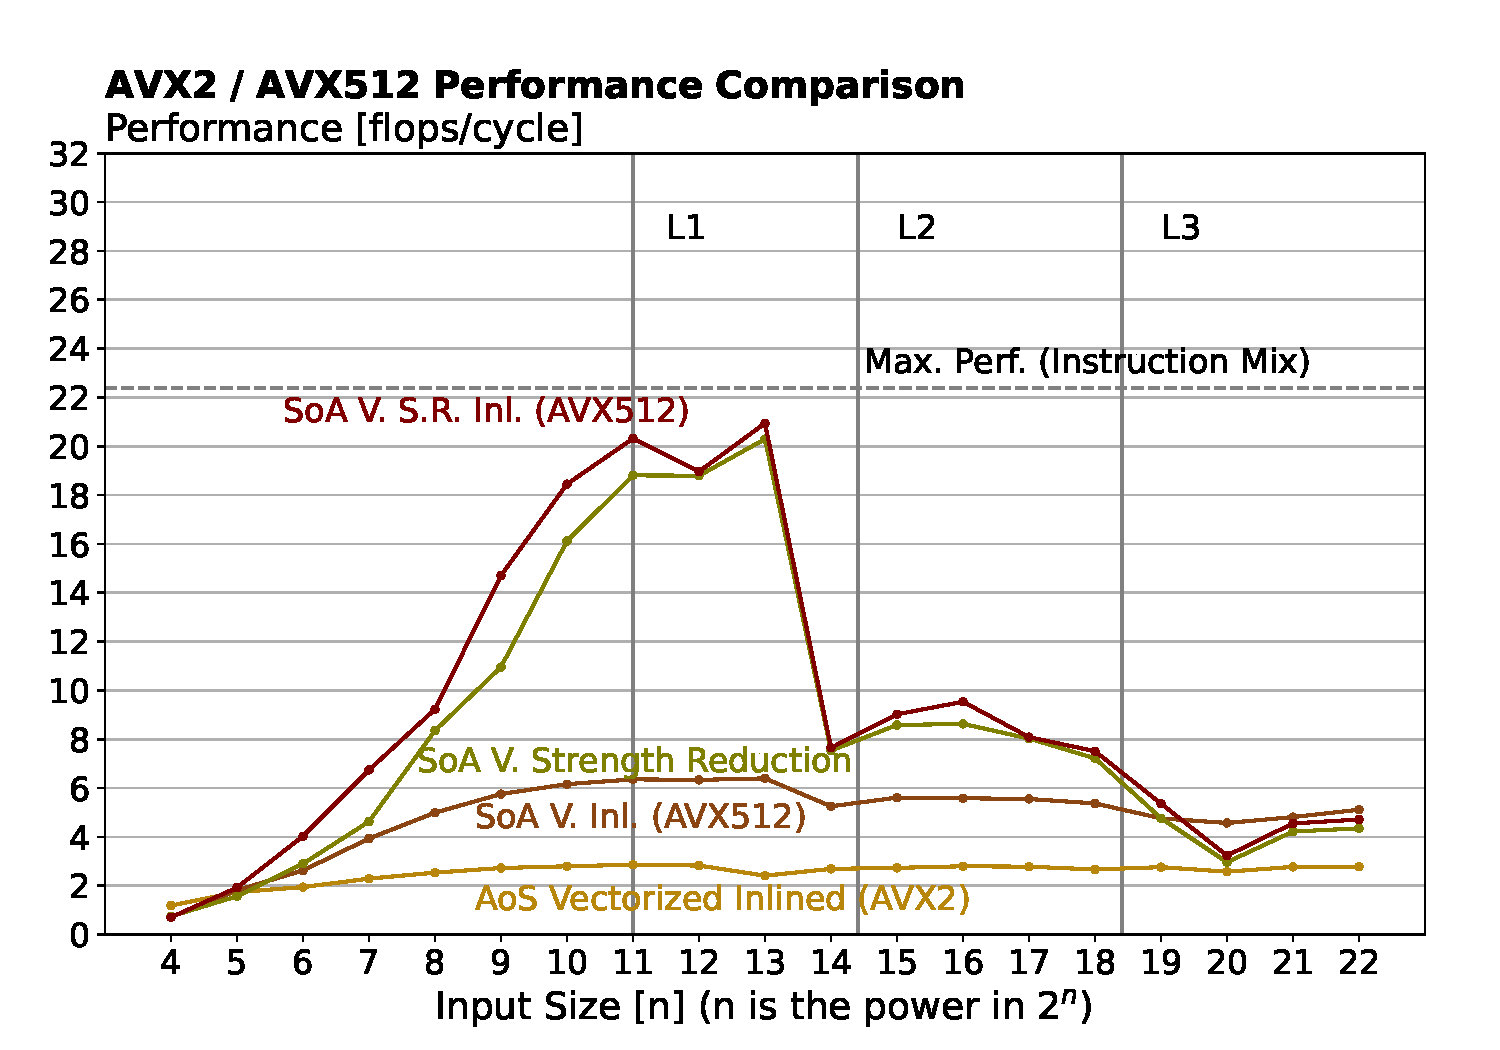
\includegraphics[scale=0.33]{gjk_performance_avx.pdf}}
%  \caption{ Performance plots for single-precision implementations of GJK. \label{gjkperformance}}
%\end{figure*}

\mypar{Experimental Setup for BVH}
We conducted our experiments for BVH using a server with an Intel Xeon \texttt{D-2141I} CPU (Skylake Server architecture).
It has a nominal base frequency of $2.20$ GHz. % , but was fixed to $1.0$ GHz on the rented server
The cache sizes for L$1$, L$2$ and L$3$ caches are $64$ KiB ($32$ KiB \textbf{I} + $32$ KiB \textbf{D}) per core, $1$ MiB per core and $11$ MiB (shared) respectively.
L$1$ cache is $8$-way set associative, L$2$ cache is $16$-way set associative and L$3$ is $11$-way associative.
To compile our code we used GCC version $11.1$.
The optimization flags we used are \texttt{-std=c11 -march=skylake-avx512 -mprefer-vector-width=512 -ffast-math}.
The experiments were conducted using \textbf{cold} cache.
Warm cache isn't representative (one wouldn't repeat the exact same collision test more than once).

As input, we imported two high-resolution $3$D models (in .OBJ format) and set up two scenes: where the objects intersect and where they don't intersect.
To try and somewhat control for the algorithm's dependence on scene geometry, we decided to generate the both scenes each at multiple resolutions, using Blender's "Decimate Geometry" modifier \cite{blender}.
The full-resolution scenes have $\approx 5.4$M triangles total, and we generated scenes in resolutions from $10\%, 20\%, ..., 90\%, 100\%$.
%All scenes are significantly larger cache sizes, and even the $10\%$ scene doesn't fit in any cache.
%BVH does not see significant speedup for cache-fitting scenes, to the point where a $1$K triangles scene (sphere inside concave shell) can take similar time to a $\approx 1.8$M triangle scene ($30\%$ resolution).

\mypar{Results (BVH)} Many of the results obtained cannot be immediately explained by a typical performance analysis.
Rather, it is helpful to look at the number of triangle-triangle tests performed, shown in Fig. \ref{bvhtriangles}.
In the following, we will keep referring back to the triangle-triangle test number when discussing the results.

\begin{figure}[!ht]
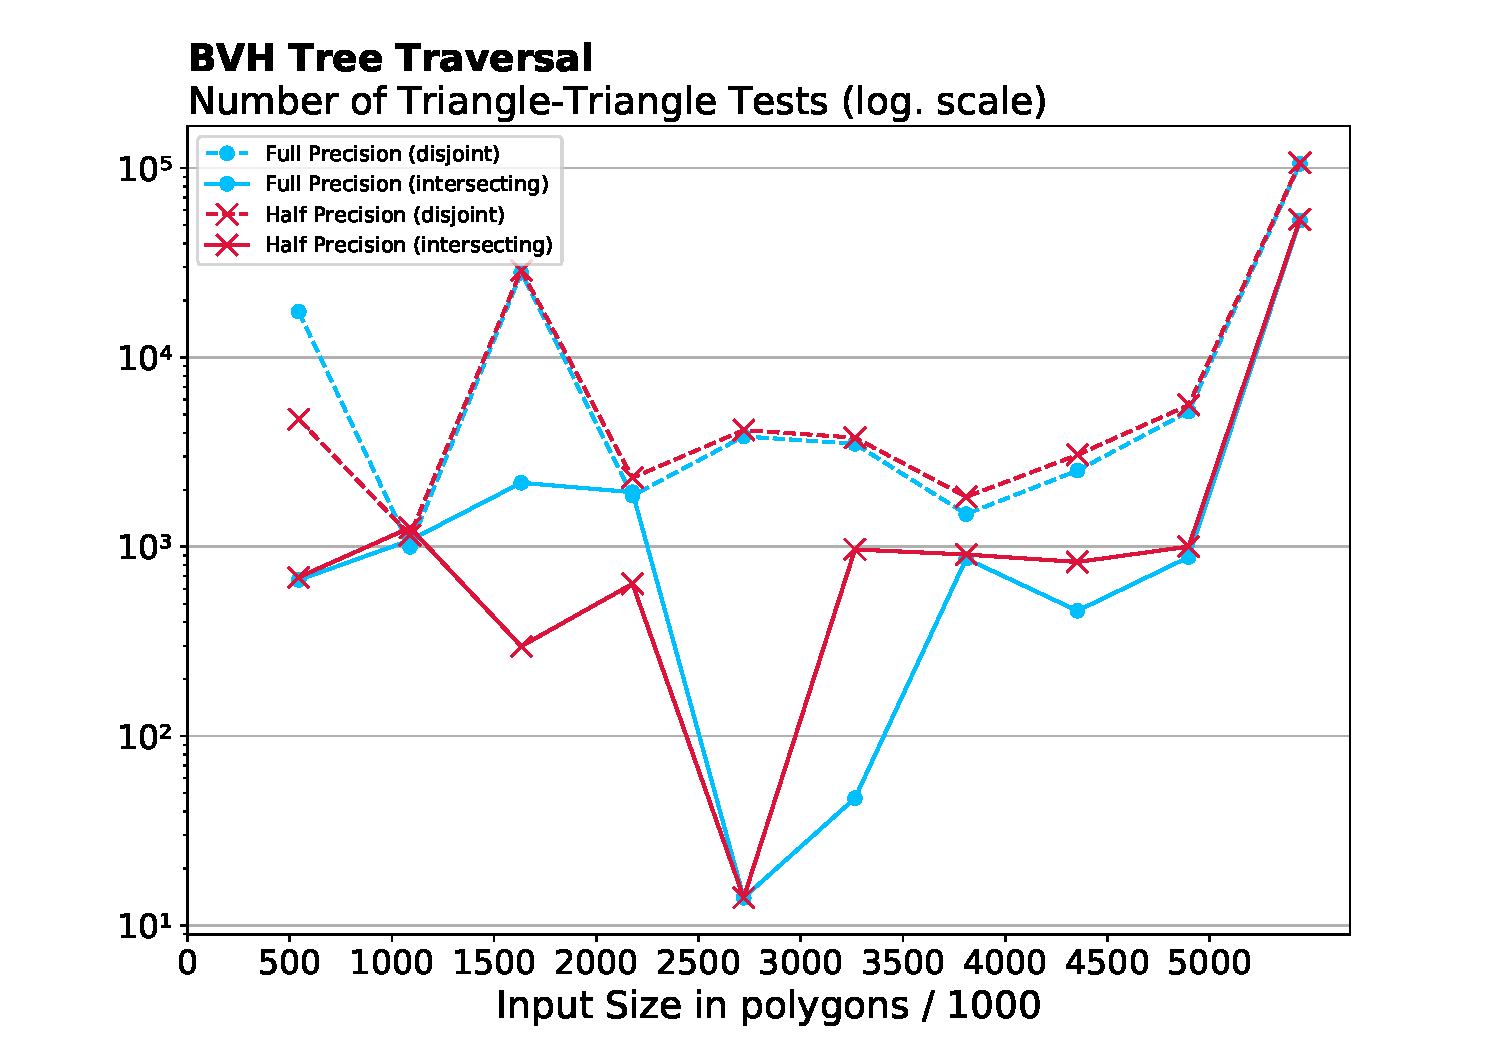
\includegraphics[width=1.1\linewidth]{bvh_triangles.pdf}
\caption{Number of triangle-triangle tests performed during BVH traversal.}
\label{bvhtriangles}
\end{figure}

Fig. \ref{bvhcycles} shows the runtime in cycles for each BVH version, as a function of \# Triangles in the Scenes. 
We see fairly uniform runtimes, even as the input sizes vary by millions of triangles.
The one exception is a $4\times$ (disjoint) or $10\times$ spike (intersecting) in runtime for the $100\%$ scene.
The main reason is that we also perform $20\times$ (disjoint) or $60\times$ (intersecting) more triangle tests.
We suspect that Blender's "decimate geometry" is very beneficial to the convergence of Neural Gas during tree construction.
The intersecting case generally takes an order of magnitude less cycles, with a similar decrease in triangle-triangle tests.

\begin{figure}[!ht]
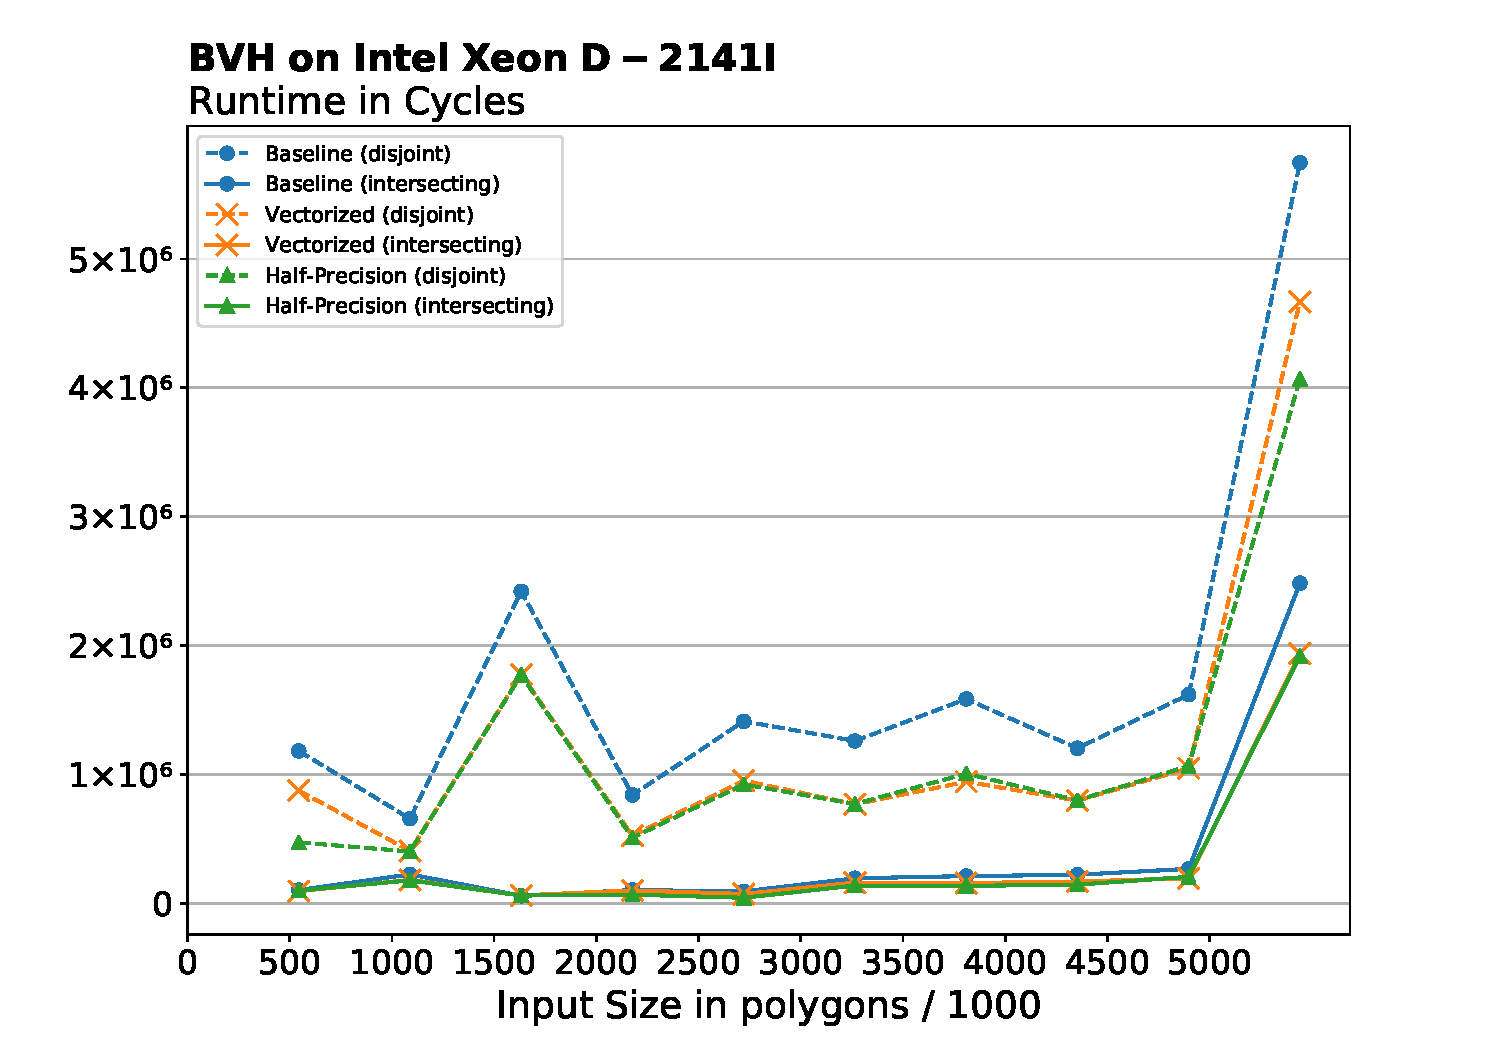
\includegraphics[width=1.1\linewidth]{bvh_cycles.pdf}
\caption{Runtime of BVH in cycles for all optimizations and both intersecting and disjoint scenes.}
\label{bvhcycles}
\end{figure}

Fig. \ref{bvhperformance} shows the performance in \texttt{flops}$/$\texttt{cycles} of BVH.
Within each optimization level and scene-type (intersecting or not), performance is fairly consistent.
As a greater proportion of time is spent traversing trees when the objects are apart, we also see the largest performance increase.
Vectorized code achieved almost a $3\times$ performance increase at $\approx 1.4$ \texttt{flops/cycle}.
An even larger increase was reached via quantization: over $4\times$.
However, those performance increases are \textbf{misleading}, as the runtime speedup is only around $1.6\times$.
To explain this, recall that baseline implementation does not have to test all kDOP directions in case it finds non-overlap along one of them.
Both vectorized and quantized code do not have this "early stopping" so they perform more flops for the same result.

\begin{figure}[!ht]
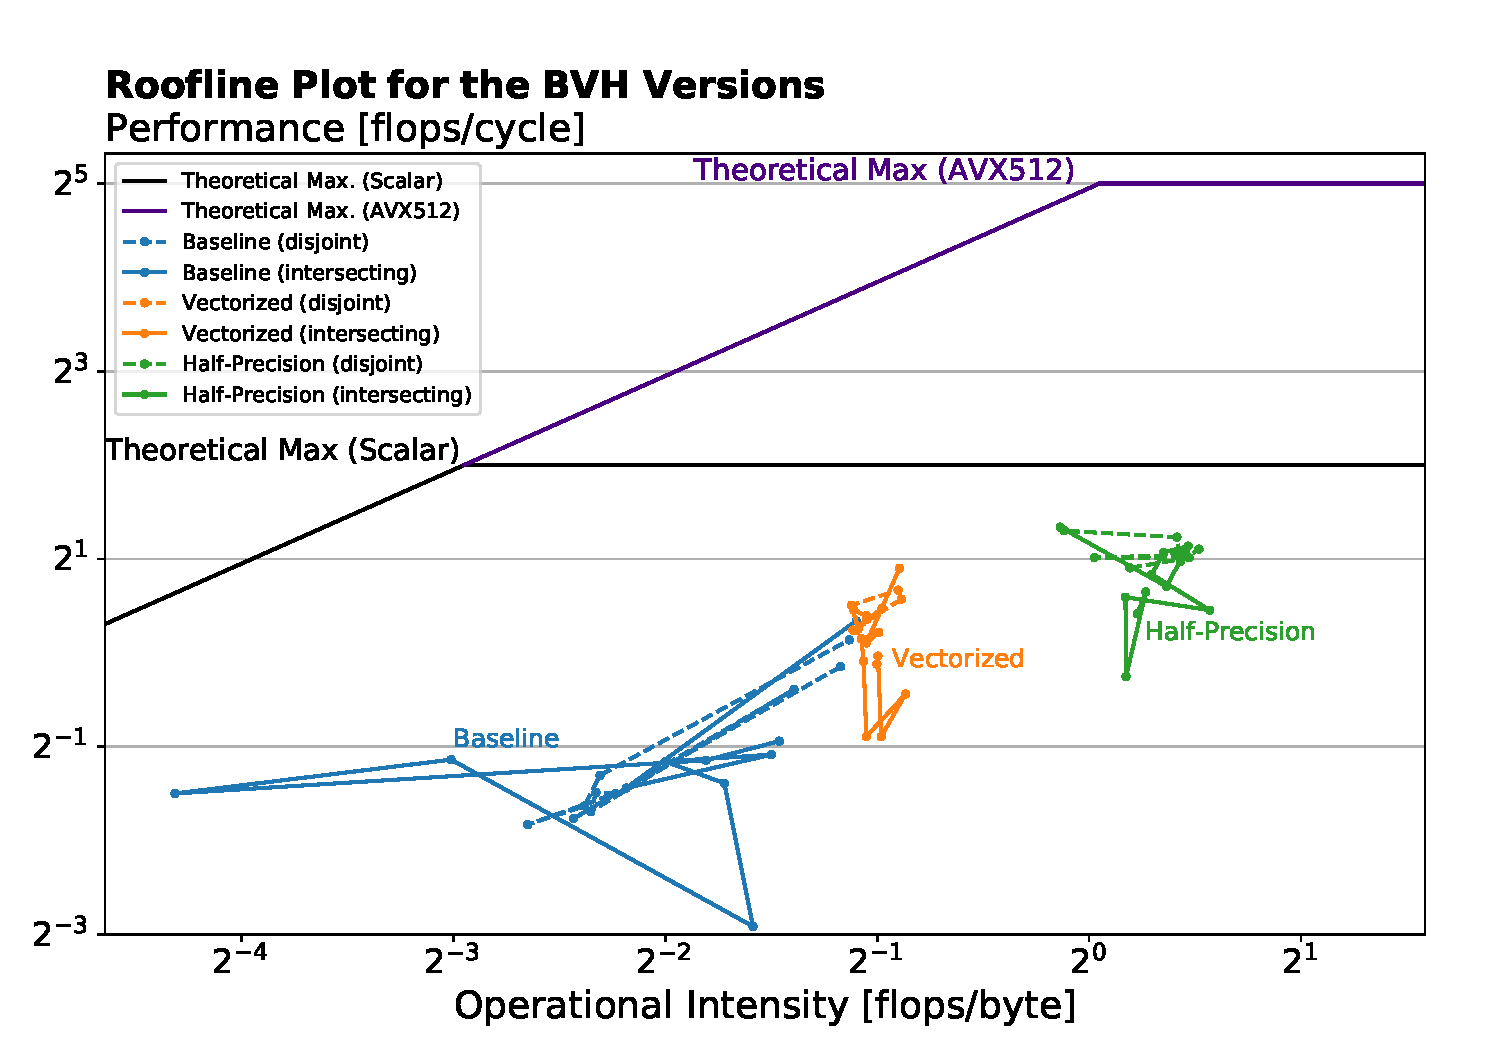
\includegraphics[width=1.05\linewidth]{bvh_roofline.pdf}
\caption{Roofline plot for the BVH optimizations in both scenes. Vectorized code has $\approx 2\times$ and quantized code $\approx 3\times$ the flops of baseline.}
\label{bvhroofline}
\end{figure}

Looking at the roofline plot in Fig. \ref{bvhroofline}, we see that indeed most BVH runs were memory bound.
Only half-precision quantized code - and only for half the input scenes - is barely compute bound.
The around $2\times$ operational intensity of half-precision vs. vectorized fp32 is a clear consequence of moving $\approx$ half the data per node.
Interestingly, operational intensity remains consistent for each optimization level, across sizes and even intersecting and disjoint scenes.
This is in contrast to the runtime (and to a lesser extent performance) differences between the intersecting and disjoint scenes.

\begin{figure}[!ht]
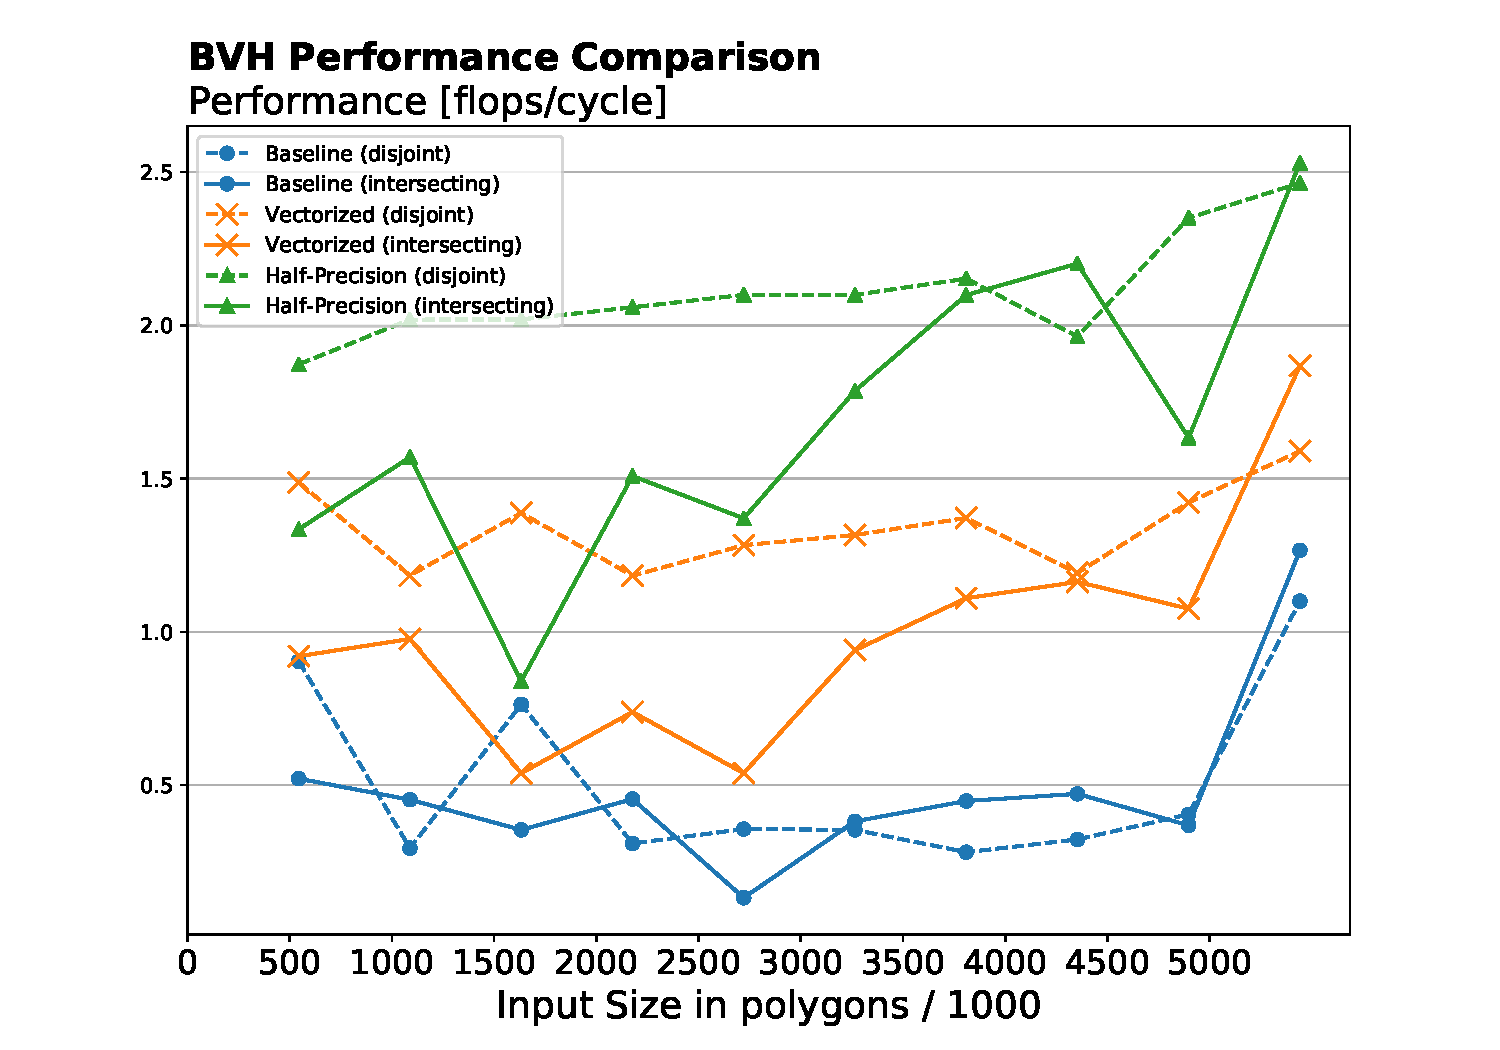
\includegraphics[width=1.1\linewidth]{bvh_performance.pdf}
\caption{Performance of the BVH optimizations, for both intersecting and disjoint scenes.}
\label{bvhperformance}
\end{figure}



%Here you evaluate your work using experiments. You start again with a
%very short summary of the section. The typical structure follows. 

%\mypar{Experimental setup} Specify the platform (processor, frequency, cache sizes)
%as well as the compiler, version, and flags used. I strongly recommend that you play with optimization flags and consider also icc for additional potential speedup.

%Then explain what input you used and what range of sizes. The idea is to give enough information so the experiments are reproducible by somebody else on his or her code.

%\mypar{Results}
%Next divide the experiments into classes, one paragraph for each. In the simplest case you have one plot that has the size on the x-axis and the performance on the y-axis. The plot will contain several lines, one for each relevant code version. Discuss the plot and extract the overall performance gain from baseline to best code. Also state the percentage of peak performance for the best code. Note that the peak may change depending on the situation. For example, if you only do additions it would be 12 Gflop/s
%on one core with 3 Ghz and SSE and single precision floating point.

%Do not put two performance lines into the same plot if the operations count changed significantly (that's apples and oranges). In that case first perform the optimizations that reduce op count and report the runtime gain in a plot. Then continue to optimize the best version and show performance plots.

%{\bf You should}
%\begin{itemize}
%\item Follow to a reasonable extent the guide to benchmarking presented in class, in particular
%\item very readable, attractive plots (do 1 column, not 2 column plots
%for this class), proper readable font size. An example is below (of course you can have a different style),
%\item every plot answers a question, which you pose and extract the
%answer from the plot in its discussion
%\end{itemize}
%Every plot should be referenced and discussed (what does it show, which statements do
%you extract).

\section{Conclusions}
We have presented optimized implementations of two collision detection algorithms:  The Gilbert-Johnson-Keerthi Algorithm (GJK) and Bounding Volume Hierarchies (BVH).

The best performing implementation of GJK gave a $13.5\times$ speedup compared to the baseline implementation, performing close to the theoretical peak of $22.4$ flops/cycle. SoA format and the use of AVX-512 gave the biggest improvement in performance.

For BVH, performance and cycle count depend more on underlying geometry. We achieve a maximal speedup of $2.45\times$ (with an up-to $8\times$ increase in performance).
Performance was below peak, due to the poor locality and "pointer-chasing" nature of tree traversal.

Future work could further parallelize intersection testing (GJK and BVH traversal) by utilizing multiple cores (or even GPUs).
And with ever-wider vector registers, the tree arity on BVH trees could further be increased for even better performance.


%Here you need to briefly summarize what you did and why this is
%important. {\em Do not take the abstract} and put it in the past
%tense. Remember, now the reader has (hopefully) read the paper, so it
%is a very different situation from the abstract. Try to highlight
%important results and say the things you really want to get across
%(e.g., the results show that we are within 2x of the optimal performance ...
%Even though we only considered the DFT, our optimization
%techniques should be also applicable ....) You can also formulate next
%steps if you want. Be brief.
%
%\section{Further comments}
%
%Here we provide some further tips.
%
%\mypar{Further general guidelines}
%
%\begin{itemize}
%\item For short papers, to save space, I use paragraph titles instead of
%subsections, as shown in the introduction.
%
%\item It is generally a good idea to break sections into such smaller
%units for readability and since it helps you to (visually) structure the story.
%
%\item The above section titles should be adapted to more precisely
%reflect what you do.
%
%\item Each section should be started with a very
%short summary of what the reader can expect in this section. Nothing
%more awkward as when the story starts and one does not know what the
%direction is or the goal.
%
%\item Do not use subsubsections.
%
%\item Make sure you define every acronym you use, no matter how
%convinced you are the reader knows it.
%
%\item Always spell-check before you submit.
%
%\item Be picky. When writing a paper you should always strive for 
%high quality. Many people may read it and the quality makes a big difference.
%In this class, the quality contributes to the grade.
%\end{itemize}
%
%\mypar{Graphics} For plots that are not images {\em never} generate (even as intermediate step)
%jpeg, gif, bmp, tif. Use eps, which means encapsulate postscript, or pdf. This way it is
%scalable since it is a vector graphic description of your graph. E.g.,
%from Matlab, you can export to eps or pdf.
%
%Fig.~\ref{fftperf} is an example plot that I used in a lecture. Note that the fontsize in the plot should not be any smaller. On the other hand it is also a good rule that the font size in the plot is not larger than the one in the caption (otherwise it looks ugly).
%
%\bigskip
%{\bf Up to here you have 8 pages.}

\section{Contributions of Team Members}

%In this mandatory section (which is not included in the 8 pages limit) each team member should very briefly (telegram style is welcome) explain what she/he did for the project. I imagine this section to be between one column and one page (absolute maximum).
%
%Include only 
%\begin{itemize}
%	\item What relates to optimizing your chosen algorithm / application. This means writing actual code for optimization or for analysis.
%	\item What you did before the submission of the presentation.
%\end{itemize}
%Do not include
%\begin{itemize}
%	\item Work on infrastructure and testing.
%	\item Work done after the presentation took place.
%\end{itemize}
%
%Example and structure follows.

\subsection{Mihai} Created the Baselines for both GJK and BVH.
Implemented all BVH optimizations (vectorization, quantization, recursion).
Instrumented BVH code for profiling and analysis.
Collected cycle, flop count and data movement information for BVH.
Plotted the speedup, performance and roofline models for the BVH implementations.

\subsection{Berke} Implemented the initial baseline for GJK.
Focused on GJK optimizations and analysis. Did the profiling, bandwidth/data trasfer and locality analysis for baseline GJK implementation.
Implemented all of the standard C optimizations and vectorized versions of GJK.
Collected the cycle and flop count information for the plots by instrumenting the code.
Plotted the speedup, performance and roofline models for the GJK implementations.

\subsection{Chris}
Analyzed BVH Triangle-Triangle collision for optimization potential.
Contributed to runtime measurement framework BVH:
E.g. mesh loading/conversion, added cube and sphere collision test cases.
Multiresolution runtime tests with Mihai.
Investigated BVH runtime instabilities.
Created interactive 3d visualizations GJK and BVH to aid analysis and verification of performance bottlenecks, correctness and runtime stability.

\subsection{Liam} Implemented random GJK test cases for profiling optimizations. Collected cycle and flop count information for BVH performance plots. Worked on triangle-triangle optimization for BVH.

% References should be produced using the bibtex program from suitable
% BiBTeX files (here: bibl_conf). The IEEEbib.bst bibliography
% style file from IEEE produces unsorted bibliography list.
% -------------------------------------------------------------------------
\bibliographystyle{IEEEbib}
\bibliography{bibl_conf}


\end{document}
